\section{Data Processing}
\label{sec:data-processing}

\subsection{Principal Components Analysis (PCA)}
\label{sec:data-processing:pca}

The task is to train a model on the training dataset and predict on a noised test dataset.
The training set has 6666 pictures, while the test set have 2857 pictures.
Each picture has 1536 features.
This feature dimension is too large for models.
Therefore, I use principal components analysis (PCA) to reduce the dimension of features.
The steps of PCA are as follows:
\begin{enumerate}
    \item Substrate the mean value of each feature.
    \item Compute the covariance matrix with python function $np.cov$.
    \item Compute the covariance matrix's eigenvalue and eigenvector with python function $np.linalg.eig$, and sort the eigenvalue in descending order.
    \item Keep the first $N$ columns of eigenvectors, and use the $1536\times N$ submatrix to map the features from the original space to the new space.
\end{enumerate}

One key value to decide is the dimension of the new space $N$.
We use the following equation to compute the error of PCA:
\begin{equation}
    1 - \dfrac{\sum_{i=0}^N \lambda_i}{\sum_{i=0}^{1536} \lambda_i} < \varepsilon
    \label{eqn:pca-error}
\end{equation}
Where $\lambda_i$ is the $i^\mathrm{th}$ eigenvalue of the covariance matrix.
We set $\varepsilon=0.3$, and from \figurename{}~\ref{fig:pca}, the corresponding $N=112$.

\begin{figure}
    \centering
    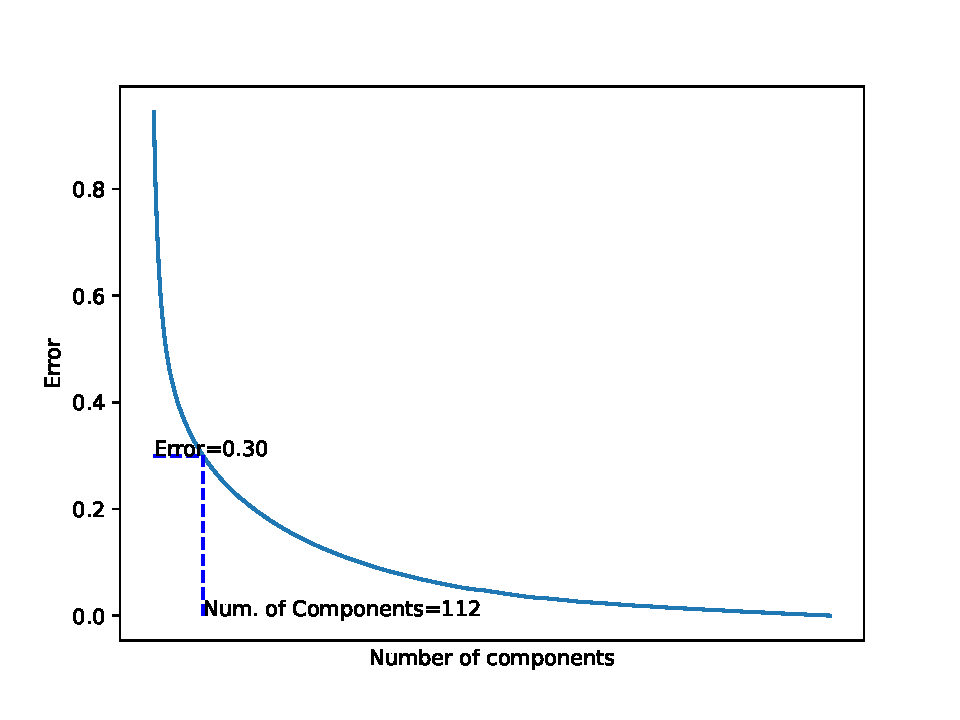
\includegraphics[width=0.9\linewidth]{figures/pca_components.pdf}
    \caption{Relationship between PCA error and the dimension of the new space $N$}
    \label{fig:pca}
\end{figure}


\subsection{Reduced Rank Linear Discriminant Analysis (Reduced Rank LDA)}
\label{sec:data-processing:rr-lda}

Another method to reduce the dimension is Reduced Rank Linear Discriminant Analysis (Reduced Rank LDA).
Unlike PCA, Reduced Rank LDA tries to find the discriminant direction which minimizes this overlap for Gaussian data.
The step is as follows:
\begin{enumerate}
    \item Estimate the centroid matrix $M_{k\times P}$, and the variance of the sample $W=\hat{\Sigma}$.
    \item Compute $M^*=MW^{-1/2}$.
    \item Compute $B^*$, the covariance matrix of $M^*$, and compute the eigenvector matrix $V^*$.
    \item The new discriminant variable is $Z_l=v_l^TX$, with $v_l=W^{-1/2}v_l^*$
\end{enumerate}

Note that the Reduced Rank LDA can only reduce the number of dimensions to $L-1$ dimensions, with $L=20$ being the number of classes.
Therefore, compared to PCA, Reduced Rank LDA loses too much information.
We will discuss this in the experiment Section \ref{sec:model-selection}.